% =====================================================================
%  Informe final - Tarea Académica 1
%  Deep Learning para Finanzas (1FIN58) - PUCP
%  Compilar con pdflatex (dos pasadas). Las figuras van en ./figuras/
% =====================================================================
\documentclass[12pt,a4paper]{article}

% ---------- Idioma y tipografía ----------
\usepackage[utf8]{inputenc}
\usepackage[T1]{fontenc}
\usepackage[spanish,es-noshorthands,es-tabla]{babel}
\usepackage{mathptmx}            % Times
\usepackage{microtype}
\usepackage{amsmath,amssymb}
\usepackage{courier}             % monoespaciada Type 1

% ---------- Página ----------
\usepackage[margin=2.5cm]{geometry}
\usepackage{setspace}
\onehalfspacing
\setlength{\parindent}{1.25cm}
\setlength{\parskip}{0pt}

% ---------- Tablas, figuras y leyendas ----------
\usepackage{graphicx}
\graphicspath{{figuras/}}
\usepackage{booktabs}
\usepackage{tabularx}
\usepackage{longtable}
\usepackage{threeparttable}
\usepackage{float}
\usepackage{array}
\usepackage{multirow}
\usepackage[labelfont=bf,textfont=it,labelsep=newline,singlelinecheck=false,
            justification=raggedright,skip=4pt,font=small]{caption}
\captionsetup[table]{position=top}
\captionsetup[figure]{position=top}

% ---------- Encabezados ----------
\usepackage{titlesec}
\titleformat{\section}{\normalfont\large\bfseries\centering}{\thesection.}{0.5em}{}
\titleformat{\subsection}{\normalfont\normalsize\bfseries}{\thesubsection}{0.5em}{}
\titleformat{\subsubsection}{\normalfont\normalsize\bfseries\itshape}{\thesubsubsection}{0.5em}{}
\titlespacing*{\section}{0pt}{18pt}{8pt}
\titlespacing*{\subsection}{0pt}{12pt}{4pt}

\usepackage{fancyhdr}
\pagestyle{fancy}
\fancyhf{}
\fancyhead[L]{\small\scshape Tarea Académica 1 — Riesgo de impago}
\fancyhead[R]{\small\thepage}
\renewcommand{\headrulewidth}{0.3pt}

\usepackage{enumitem}
\setlist{itemsep=2pt,topsep=4pt}
\usepackage[hidelinks]{hyperref}

\newcommand{\nota}[1]{\par\vspace{2pt}{\footnotesize\textit{Nota.} #1\par}}
\newcommand{\code}[1]{\texttt{#1}}

% =====================================================================
\begin{document}

% ---------------------------- Portada --------------------------------
\begin{titlepage}
\thispagestyle{empty}
\centering
{\large\scshape Pontificia Universidad Católica del Perú\par}
\vspace{0.3cm}
{\normalsize Deep Learning para Finanzas (1FIN58)\par}
\vspace{3.2cm}
\rule{\linewidth}{0.8pt}\par\vspace{0.5cm}
{\LARGE\bfseries Predicción de impago en préstamos\\[0.2cm] de Lending Club con redes neuronales\par}
\vspace{0.5cm}
{\large Búsqueda secuencial de hiperparámetros, comparación\\ con modelos base e interpretabilidad\par}
\vspace{0.4cm}\rule{\linewidth}{0.8pt}\par
\vspace{1.2cm}
{\large Informe final — Tarea Académica 1\par}
\vfill
{\large Sebastián Estefano Hernández Muñaqui\par}
\vspace{0.3cm}
{\normalsize [Integrantes del grupo]\par}
\vspace{1.2cm}
{\normalsize Lima, octubre de 2026\par}
\end{titlepage}

% ---------------------------- Resumen --------------------------------
\section*{Resumen}
\addcontentsline{toc}{section}{Resumen}
\noindent Se entrenaron redes neuronales densas para predecir si un préstamo de Lending Club termina en impago (\textit{Charged Off}, 14.8\,\% de los casos) y se compararon con regresión logística, árbol de decisión y \textit{Random Forest}. Antes de la búsqueda se corrigieron dos problemas del avance inicial: el MinMaxScaler no llegaba a los modelos y, por el desbalance de clases, las redes respondían «pagado» para todos los préstamos (exactitud de 85\,\% con F1 igual a cero). La búsqueda se hizo de forma secuencial, un hiperparámetro por etapa, en el orden optimizador $\rightarrow$ tasa de aprendizaje $\rightarrow$ tamaño de lote $\rightarrow$ activación $\rightarrow$ capas $\rightarrow$ neuronas $\rightarrow$ distribución de neuronas $\rightarrow$ \textit{dropout} $\rightarrow$ regularización $\rightarrow$ \textit{early stopping} $\rightarrow$ épocas, eligiendo en cada etapa la mejor precisión promedio (AP) de validación. Se evaluaron 43 configuraciones en unos 73 minutos. La red final tiene 20 capas de 64 neuronas con activación tanh, Adam con tasa de 0.0001, lote 32, \textit{dropout} 0.25 y L1 de $10^{-4}$. A diferencia de la corrida anterior, ya no se sobreajusta: su AUC es 0.683 en entrenamiento, 0.690 en validación y 0.675 en prueba. Sin embargo, no supera a los modelos base. En prueba, con el umbral elegido en validación, todos los modelos competitivos quedan en un AUC de 0.675--0.677 y un F1 de 0.33--0.34; el modelo seleccionado solo con validación fue la regresión logística balanceada (AUC 0.677, AP 0.270, F1 0.339). Las tres técnicas de interpretabilidad coinciden en que el plazo, la tasa de interés y el grado crediticio son las variables que más empujan el riesgo.

\vspace{0.3cm}
\noindent\textbf{Palabras clave:} riesgo de crédito, redes neuronales, desbalance de clases, búsqueda de hiperparámetros, SHAP.

\newpage
\tableofcontents
\newpage

% =====================================================================
\section{Introducción}

El objetivo de la tarea es diagnosticar y mejorar una red neuronal que predice el estado final de un préstamo: \textit{Fully Paid} (0) o \textit{Charged Off} (1). El problema tiene una dificultad central: solo el 14.8\,\% de los préstamos termina en impago. Por eso, un modelo que diga siempre «pagado» alcanza una exactitud de 85.2\,\% sin detectar un solo impago. La exactitud, por sí sola, no sirve para evaluar estos modelos, y el informe se apoya en métricas que miran a la clase minoritaria: F1, precisión promedio (AP) y AUC ROC.

El informe documenta el notebook final con las etapas reordenadas (versión v3), ejecutado en su modalidad extensa. La Sección~\ref{sec:datos} describe los datos y los problemas del avance inicial; la Sección~\ref{sec:metodo}, las métricas y el diseño de la búsqueda; la Sección~\ref{sec:busqueda}, los resultados etapa por etapa; la Sección~\ref{sec:comparacion}, la comparación con los modelos base; la Sección~\ref{sec:interp}, la interpretabilidad; la Sección~\ref{sec:discusion}, la discusión; la Sección~\ref{sec:sirve}, si la red sirve para este problema y cómo continuar; y la Sección~\ref{sec:conclusiones}, las conclusiones.

% =====================================================================
\section{Datos y preprocesamiento}\label{sec:datos}

\subsection{Base de datos y partición}

La base contiene 19\,908 préstamos. Se excluyeron 3 filas cuya etiqueta estaba vacía o no era reconocida; en el avance inicial esas filas se convertían artificialmente en \textit{Fully Paid}. Se construyeron dos variables: la antigüedad laboral en años (\code{emp\_length\_numeric}) y el año de emisión (\code{issue\_year}). Se eliminaron identificadores y columnas de texto libre (\code{index}, \code{emp\_title}, \code{emp\_length} original, \code{issue\_d} y \code{pymnt\_plan}).

La partición es estratificada: primero se separa 20\,\% para prueba y luego 20\,\% del resto para validación, lo que da 64\,\%, 16\,\% y 20\,\% (Tabla~\ref{tab:particion}). La proporción de impagos es la misma en los tres conjuntos, y por eso el modelo trivial obtiene 85.2\,\% en todos.

\begin{table}[H]
\caption{Partición estratificada de la base}\label{tab:particion}
\centering
\begin{tabular}{lrrr}
\toprule
Conjunto & Filas & Proporción de impago & Exactitud de «siempre 0» (\%) \\
\midrule
Entrenamiento & 12\,739 & 0.1478 & 85.22 \\
Validación    &  3\,185 & 0.1479 & 85.21 \\
Prueba        &  3\,981 & 0.1480 & 85.20 \\
\bottomrule
\end{tabular}
\nota{La prueba se consulta solo después de congelar modelos y umbrales.}
\end{table}

\subsection{Problema inicial 1: el MinMaxScaler no se aplicaba}

En el avance inicial, el MinMaxScaler (y un RobustScaler) se construían usando la matriz de variables antes de que esta existiera, y sus salidas nunca se pasaban a los modelos. En la práctica, las redes se entrenaban sin el escalado previsto. Esto importa porque las variables tienen escalas muy distintas: el ingreso anual está en decenas de miles y la tasa de interés en unidades. Sin escalar, la red da más peso a los números grandes solo por su magnitud y el descenso por gradiente se vuelve inestable. Además, la imputación de valores faltantes se ajustaba con toda la base, lo que filtraba información de validación y prueba hacia el entrenamiento.

La corrección fue un único preprocesador (\code{ColumnTransformer}) que se \textbf{ajusta solo con entrenamiento} y luego se aplica a validación y prueba. Las variables numéricas se imputan con la mediana y se llevan al rango $[0,1]$ con MinMaxScaler; las categóricas se imputan con la moda y se codifican en \textit{one-hot}. Resultan 49 variables de entrada: 12 numéricas y 37 indicadoras. Los valores de validación o prueba pueden quedar ligeramente fuera de $[0,1]$ si superan los extremos de entrenamiento; el escalador no se reajusta.

\subsection{Problema inicial 2: desbalance de clases y \texttt{class\_weight}}\label{sec:classweight}

Los resultados guardados del avance mostraban una exactitud de validación de 0.852 con precisión, \textit{recall} y F1 iguales a cero en las redes de 5, 10, 20, 50 y 100 capas. Con ambas clases presentes, esto solo es posible si la red predice la clase 0 para todos los préstamos. Con 85\,\% de casos pagados, minimizar la pérdida empuja las probabilidades por debajo de 0.5 y la regla de decisión nunca marca un impago.

Para compensarlo se calcularon pesos de clase con \code{compute\_class\_weight} de scikit-learn (Pedregosa et al., 2011) sobre el entrenamiento: 0.587 para los pagados y 3.383 para los impagos, de modo que equivocarse con un impago «cuesta» casi seis veces más. La Sección~\ref{sec:basica} muestra que estos pesos resuelven el F1 con umbral 0.5, pero que el criterio de selección los descarta porque no mejoran la capacidad de ordenar los préstamos.

% =====================================================================
\section{Metodología}\label{sec:metodo}

\subsection{Métricas}

La pérdida reportada es la entropía cruzada binaria (\textit{log-loss}) sin ponderar, comparable entre todos los modelos. Se reportan además la exactitud (\%), la exactitud balanceada, la precisión, el \textit{recall} y el F1 de la clase impago, el AUC ROC, el índice de Gini ($2\,\text{AUC}-1$) y la precisión promedio (AP):
\begin{equation}\label{eq:ap}
\text{AP} = \sum_{n} (R_n - R_{n-1})\,P_n ,
\end{equation}
donde $P_n$ y $R_n$ son la precisión y el \textit{recall} en el $n$-ésimo umbral. AP resume la curva precisión--\textit{recall}; su valor de referencia es la prevalencia de impago (0.148), no 0.5 (Saito \& Rehmsmeier, 2015). Tanto AP como AUC usan probabilidades y no dependen del umbral.

\subsection{Política de umbral}

Se usan dos umbrales: el fijo de 0.5 y uno propio de cada modelo que maximiza el F1 en validación. Este segundo umbral se congela y se aplica sin cambios a entrenamiento y prueba. Mover el umbral no cambia el orden de las probabilidades, por lo que deja intactos el AUC y el AP; solo cambia cuántos préstamos se marcan como impago.

\subsection{Búsqueda secuencial y orden de las etapas}

La búsqueda es secuencial (descenso por coordenadas): en cada etapa se varía un solo hiperparámetro, se elige el ganador por AP de validación (con el F1 de umbral optimizado y el AUC como desempates) y ese valor se conserva en las etapas siguientes. Todas las redes usan la misma semilla (42), una salida sigmoide y \textit{early stopping} sobre el AP de validación con restauración de los mejores pesos, salvo en las etapas que lo desactivan a propósito. El techo de épocas durante la búsqueda es 100.

El orden de las etapas se reorganizó respecto de la corrida anterior (Tabla~\ref{tab:orden}). La corrida previa fijaba primero la arquitectura y dejaba el optimizador, la tasa de aprendizaje y las épocas para el final; además, eligió 500 épocas sin \textit{early stopping} antes de probar \textit{dropout} o regularización, y la red resultante se sobreajustó (AUC de 0.996 en entrenamiento y 0.582 en prueba). En el orden nuevo, los hiperparámetros de optimización se fijan primero sobre la red básica de una capa, que entrena rápido; después se define la arquitectura; y al final se añaden las técnicas contra el sobreajuste y el presupuesto de épocas.

\begin{table}[H]
\caption{Orden de las etapas de la búsqueda y valores probados}\label{tab:orden}
\centering
\small
\begin{tabularx}{\linewidth}{clX}
\toprule
Etapa & Hiperparámetro & Valores probados \\
\midrule
0 & Balanceo de clases & sin pesos; pesos balanceados \\
1 & Optimizador & SGD; Adam; RMSprop; Momentum (SGD con 0.9) \\
2 & Tasa de aprendizaje & 0.01; 0.001; 0.0001 \\
3 & Tamaño de lote & 32; 64; 128 \\
4 & Activación oculta & ReLU; tanh; sigmoide; ELU \\
5 & Capas ocultas & 5; 10; 20; 50; 100 (64 neuronas por capa) \\
6 & Neuronas por capa & 32; 64; 128; 256; 512 \\
7 & Distribución & uniforme; creciente; decreciente (embudo); cuello de botella \\
8 & \textit{Dropout} & 0.25; 0.50 (después de cada capa oculta) \\
9 & Regularización & sin; L1 $=10^{-4}$; L2 $=10^{-4}$ \\
10 & \textit{Early stopping} & sin parada (100 épocas); paciencia 5, 10, 20, 50 \\
11 & Épocas (sin \textit{early stopping}) & 50; 100; 200 \\
\bottomrule
\end{tabularx}
\nota{La etapa 0 se ejecuta sobre la red básica (1 capa de 100 neuronas ReLU, Adam 0.001, lote 64, 10 épocas). En la etapa 7 todas las formas conservan la misma profundidad y el mismo total de neuronas.}
\end{table}

\subsection{Modelos base}

Se entrenaron regresión logística, árbol de decisión (profundidad máxima 5) y \textit{Random Forest} (150 árboles, 5 variables por división, 12 hojas como máximo), cada uno con y sin \code{class\_weight='balanced'}, sobre las mismas variables preprocesadas. Junto con la red básica y la red mejorada suman ocho modelos. El modelo final se selecciona \textbf{solo con validación}, por AP y luego por F1 con su umbral.

% =====================================================================
\section{Resultados de la búsqueda}\label{sec:busqueda}

La Tabla~\ref{tab:trayectoria} resume el ganador de cada etapa y la Tabla~\ref{tab:anexo} del Anexo contiene los 43 experimentos.

\begin{table}[H]
\caption{Ganador de cada etapa y su desempeño en validación}\label{tab:trayectoria}
\centering
\small
\begin{tabular}{llcccc}
\toprule
Etapa & Valor elegido & AP & AUC & F1 (umbral opt.) & Épocas \\
\midrule
Balanceo & sin pesos & 0.2640 & 0.6860 & 0.360 & 10 \\
Optimizador & Adam & 0.2661 & 0.6888 & 0.361 & 10 \\
Tasa de aprendizaje & 0.0001 & 0.2690 & 0.6895 & 0.366 & 48 \\
Lote & 32 & 0.2693 & 0.6899 & 0.365 & 32 \\
Activación & tanh & \textbf{0.2765} & \textbf{0.6940} & 0.366 & 63 \\
Capas & 20 & 0.2721 & 0.6836 & 0.346 & 38 \\
Neuronas & 64 & 0.2721 & 0.6836 & 0.346 & 38 \\
Distribución & uniforme & 0.2721 & 0.6836 & 0.346 & 38 \\
\textit{Dropout} & 0.25 & 0.2520 & 0.6737 & 0.351 & 25 \\
Regularización & L1 & 0.2640 & 0.6805 & 0.350 & 23 \\
\textit{Early stopping} & paciencia 5 & 0.2640 & 0.6805 & 0.350 & 23 \\
Épocas & 50 (sin parada) & 0.2627 & 0.6896 & 0.355 & 50 \\
\bottomrule
\end{tabular}
\nota{El F1 se calcula con el umbral que maximiza F1 en validación. El máximo de AP de toda la búsqueda (en negrita) se alcanzó con la red de una sola capa y activación tanh.}
\end{table}

\subsection{Red básica y balanceo}\label{sec:basica}

La red básica (1 capa de 100 neuronas ReLU, Adam 0.001, lote 64, 10 épocas) alcanza en validación un AUC de 0.686 y un AP de 0.264, claramente por encima del azar (0.5 y 0.148). Sin embargo, con umbral 0.5 predice solo 7 impagos y su F1 es 0.004: el mismo comportamiento del avance inicial, ahora explicado por el desbalance y no por un error de código (Figura~\ref{fig:basica}).

\begin{figure}[H]
\caption{Curvas de entrenamiento de la red básica}\label{fig:basica}
\centering
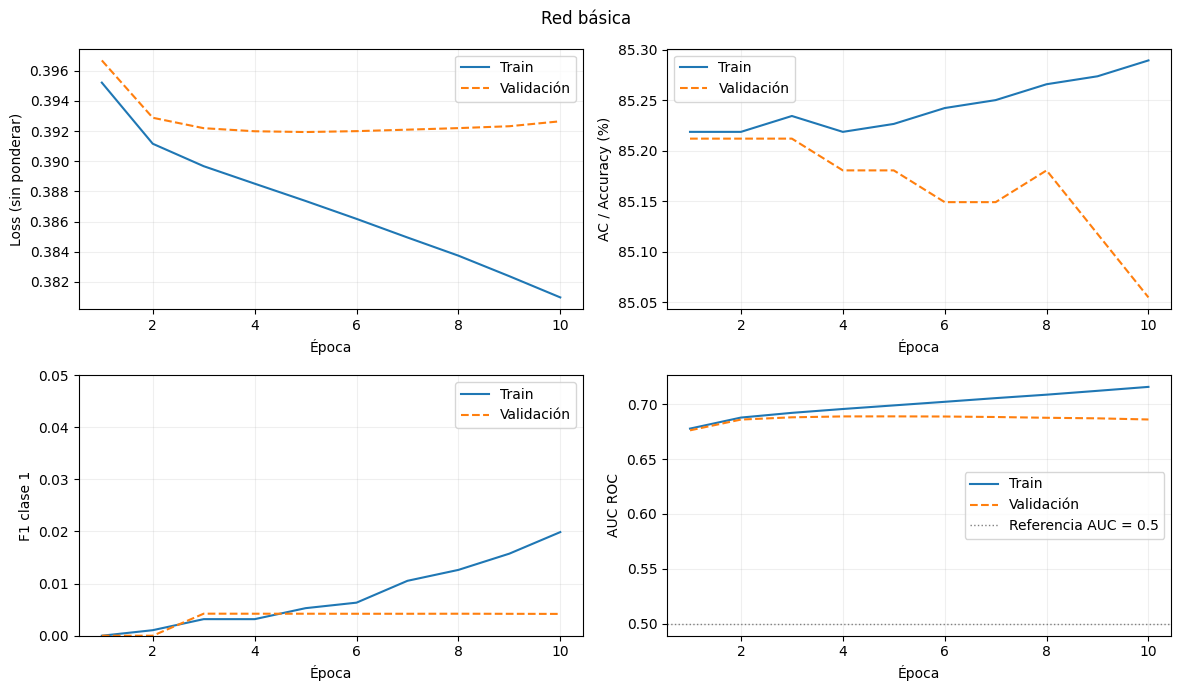
\includegraphics[width=0.88\linewidth]{c10_0.png}
\nota{Pérdida sin ponderar, exactitud, F1 de la clase impago con umbral 0.5 y AUC por época, en entrenamiento y validación.}
\end{figure}

Con pesos balanceados (Tabla~\ref{tab:balanceo}) el F1 con umbral 0.5 sube de 0.004 a 0.355 y la red marca 1\,170 impagos, a costa de bajar la exactitud a 66.8\,\%. Pero el AP prácticamente no cambia (0.2640 frente a 0.2638), porque los pesos no hacen que la red ordene mejor los préstamos: solo desplazan todas las probabilidades hacia arriba. Por una diferencia de 0.0002 se conservó la versión \textbf{sin pesos}, y desde ese punto las redes de la búsqueda vuelven a dar F1 casi nulo con umbral 0.5. El F1 con umbral optimizado confirma que pesos y umbral son casi equivalentes: 0.360 sin pesos y 0.359 con pesos.

\begin{table}[H]
\caption{Red básica sin pesos y con pesos balanceados (validación)}\label{tab:balanceo}
\centering
\begin{tabular}{lcc}
\toprule
Métrica & Sin pesos & Pesos balanceados \\
\midrule
Pérdida (sin ponderar) & 0.393 & 0.618 \\
Exactitud (\%) & 85.05 & 66.75 \\
F1, umbral 0.5 & 0.004 & 0.355 \\
Impagos predichos, umbral 0.5 & 7 & 1\,170 \\
AP & 0.2640 & 0.2638 \\
AUC & 0.6860 & 0.6835 \\
Umbral que maximiza F1 & 0.157 & 0.494 \\
F1 con ese umbral & 0.360 & 0.359 \\
\bottomrule
\end{tabular}
\end{table}

\subsection{Optimizador, tasa de aprendizaje y lote}

Con la tasa común de 0.001, Adam (Kingma \& Ba, 2015) obtuvo el mejor AP (0.2661), seguido de cerca por Momentum (0.2646) y RMSprop (0.2643). SGD sin momento quedó claramente atrás (AP 0.2366, AUC 0.666) y agotó las 100 épocas sin estabilizarse: con 0.001 avanza demasiado despacio. Esta comparación favorece a los métodos adaptativos, porque SGD suele necesitar una tasa mayor; su resultado no debe leerse como un límite del optimizador en sí.

Con Adam fijo, la tasa de 0.0001 dio el mejor AP (0.2690) y el mejor AUC (0.6895). La tasa de 0.01 detuvo el entrenamiento en 9 épocas y fue la única que marcó algunos impagos con umbral 0.5 (41), señal de pasos grandes que oscilan alrededor del mínimo. En el lote, las diferencias fueron mínimas (AP 0.2685--0.2693); se eligió 32, que además necesitó menos épocas (32) que 64 (48) y 128 (58).

\subsection{Función de activación}

Esta fue la etapa con mayor ganancia de toda la búsqueda. Tanh obtuvo AP 0.2765 y AUC 0.6940, ELU quedó prácticamente empatada (AP 0.2757, AUC 0.6937) y la sigmoide algo detrás (0.2738); ReLU fue la peor (0.2693). Con una sola capa no hay riesgo de desvanecimiento del gradiente, y las activaciones suaves (tanh, ELU) parecen ajustarse mejor a variables escaladas a $[0,1]$ y a muchas indicadoras binarias.

\subsection{Arquitectura: capas, neuronas y distribución}

Al pasar de 1 a 5 o más capas, el AP de validación \textbf{bajó} de 0.2765 a 0.262--0.272. Entre las profundidades probadas ganó 20 capas (AP 0.2721), con 5 capas cerca (0.2681). La red de 100 capas colapsó: AP 0.178, AUC 0.572 y ningún impago predicho. Sus curvas (Figura~\ref{fig:cien}) muestran una pérdida que casi no se mueve y un AUC que oscila alrededor de 0.5, el patrón típico de desvanecimiento del gradiente en redes muy profundas con tanh (Glorot \& Bengio, 2010).

\begin{figure}[H]
\caption{Curvas de entrenamiento de la red de 100 capas}\label{fig:cien}
\centering
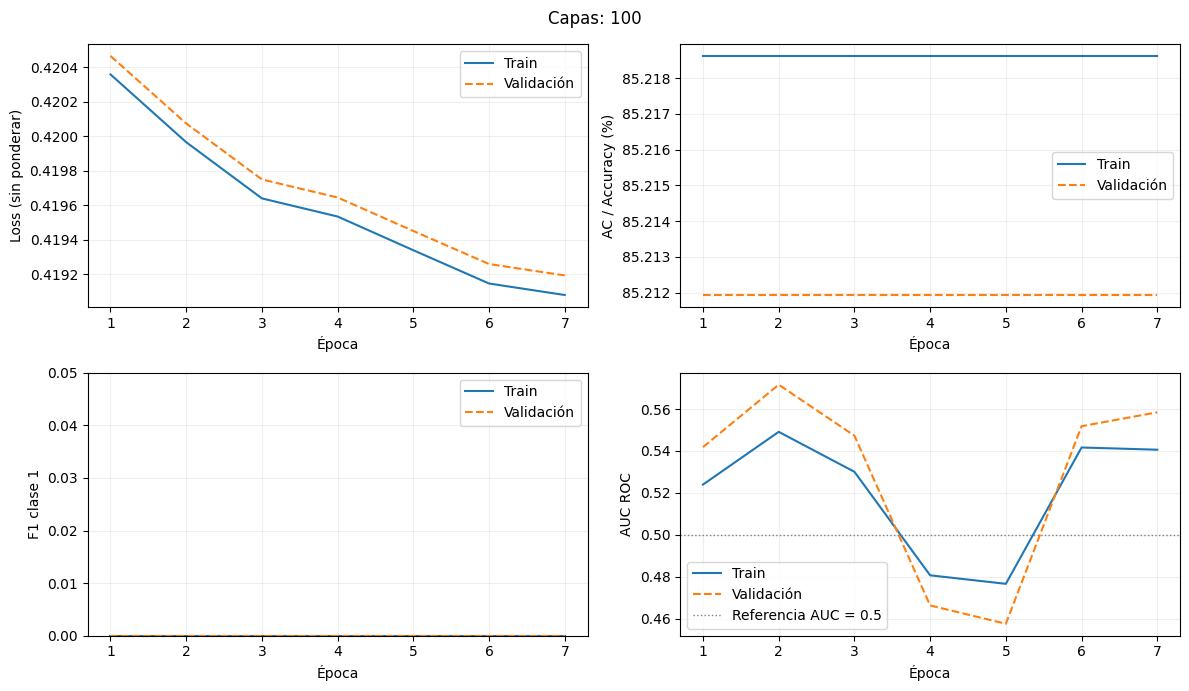
\includegraphics[width=0.85\linewidth]{c20_4.png}
\nota{La pérdida cambia en la cuarta cifra decimal y el AUC cruza la línea de 0.5; el \textit{early stopping} detuvo el entrenamiento en la época 7.}
\end{figure}

Con 20 capas fijas, el ancho de 64 neuronas fue el mejor (AP 0.2721); los anchos de 128 a 512 dejaron de predecir impagos con umbral 0.5 y se detuvieron en 6--10 épocas. En la distribución de neuronas (1\,280 neuronas en las cuatro formas), la uniforme ganó por AP (0.2721) frente al embudo (0.2636), el cuello de botella (0.2619) y la creciente (0.2437). El cuello de botella tuvo un AUC apenas mayor que la uniforme (+0.0023), pero un AP menor, por lo que no se adoptó. La arquitectura final quedó en 20 capas de 64 neuronas (82\,305 parámetros).

\subsection{\textit{Dropout}, regularización, \textit{early stopping} y épocas}

El \textit{dropout}, que apaga al azar una fracción de neuronas en cada paso de entrenamiento (Srivastava et al., 2014), empeoró la red: con 0.25 el AP cayó de 0.2721 a 0.2520 y con 0.50 la red colapsó (AP 0.167, AUC 0.543). Como la etapa no incluía la opción «sin \textit{dropout}», el procedimiento conservó 0.25 aunque fuera peor que la configuración previa (véase la Sección~\ref{sec:discusion}). La regularización L1, que penaliza la suma de los valores absolutos de los pesos (Goodfellow et al., 2016), recuperó parte de la pérdida (AP 0.2640, frente a 0.2586 con L2 y 0.2520 sin penalización).

En \textit{early stopping} (Prechelt, 1998), las cuatro paciencias restauraron los mismos pesos y dieron resultados idénticos (AP 0.2640); solo cambió el costo, de 89\,s con paciencia 5 a 251\,s con paciencia 50. Se conservó paciencia 5. Entrenar 100 épocas sin parada subió el AUC a 0.6905, pero bajó el AP a 0.2606.

La última etapa desactiva el \textit{early stopping} y compara 50, 100 y 200 épocas. Los tres valores dieron AP de 0.259--0.263 y AUC de 0.690--0.692; se eligió 50. Esta etapa solo compara entre sus propias opciones, por lo que reemplazó la configuración con paciencia 5 (AP 0.2640) por una ligeramente inferior (0.2627). A diferencia de la corrida anterior, aquí no hubo sobreajuste: las curvas de entrenamiento y validación se superponen durante las 50 épocas (Figura~\ref{fig:final}). El \textit{dropout} y la penalización L1, ya fijados en etapas previas, actúan como freno.

\begin{figure}[H]
\caption{Curvas de entrenamiento de la red mejorada final}\label{fig:final}
\centering
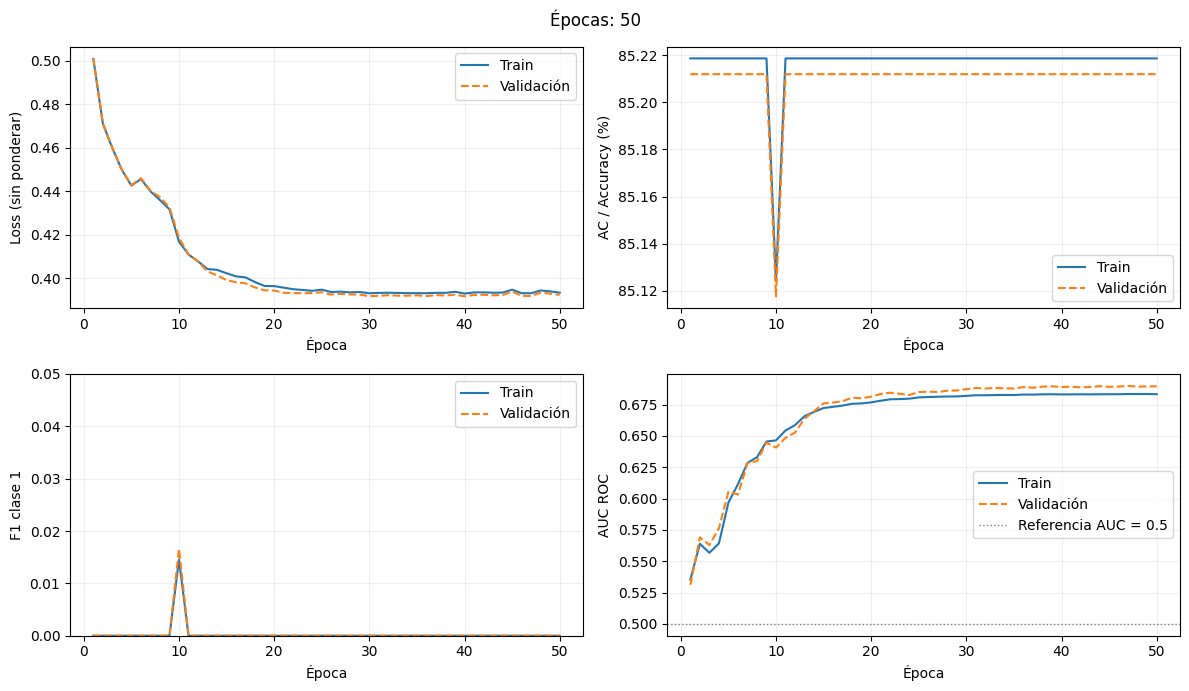
\includegraphics[width=0.88\linewidth]{c32_0.png}
\nota{20 capas de 64 neuronas tanh, Adam 0.0001, lote 32, \textit{dropout} 0.25, L1 $10^{-4}$, 50 épocas sin \textit{early stopping}. Con umbral 0.5 la red no marca impagos (F1 = 0) porque todas sus probabilidades quedan por debajo de ese valor.}
\end{figure}

\subsection{Configuración final}

La Tabla~\ref{tab:final} reúne la red básica y la red mejorada. El parche de la sección 11 del notebook, que redondea los anchos a potencias de 2, no tuvo efecto en esta corrida: la arquitectura ganadora ya era de 64 neuronas por capa, y la «Red mejorada (2\textsuperscript{n})» resultó idéntica a la red mejorada (mismos 82\,305 parámetros y mismas métricas).

\begin{table}[H]
\caption{Configuración de la red básica y de la red mejorada}\label{tab:final}
\centering
\begin{tabular}{lll}
\toprule
Hiperparámetro & Red básica & Red mejorada \\
\midrule
Capas ocultas $\times$ neuronas & $1\times100$ & $20\times64$ (uniforme) \\
Parámetros entrenables & 5\,101 & 82\,305 \\
Activación oculta & ReLU & tanh \\
Optimizador / tasa & Adam / 0.001 & Adam / 0.0001 \\
Lote & 64 & 32 \\
\textit{Dropout} & 0 & 0.25 \\
Regularización & ninguna & L1 $=10^{-4}$ \\
Épocas & 10 & 50, sin \textit{early stopping} \\
Pesos de clase & no & no \\
Umbral de validación & 0.157 & 0.178 \\
\bottomrule
\end{tabular}
\end{table}

% =====================================================================
\section{Comparación con los modelos base}\label{sec:comparacion}

\subsection{Selección en validación}

Por AP de validación, el mejor modelo base fue la \textbf{regresión logística balanceada} (AP 0.2745, AUC 0.6934), y también fue el seleccionado entre los ocho modelos, por delante de la regresión logística sin pesos (0.2732) y de la red básica (0.2640). La red mejorada obtuvo un AP de validación de 0.2627.

\subsection{Desempeño en entrenamiento, validación y prueba}

La Tabla~\ref{tab:tvt} presenta los cinco modelos principales en los tres conjuntos. La pérdida y el AUC no dependen del umbral; la exactitud y el F1 usan el umbral de validación de cada modelo.

\begin{table}[H]
\caption{Pérdida, exactitud, F1, AUC y Gini en entrenamiento, validación y prueba}\label{tab:tvt}
\centering
\small
\begin{tabular}{llccccc}
\toprule
Conjunto & Modelo & Pérdida & Exactitud (\%) & F1 & AUC & Gini \\
\midrule
\multirow{5}{*}{Entrenamiento}
 & Regresión logística   & 0.392 & 72.81 & 0.337 & 0.685 & 0.370 \\
 & Logística balanceada  & 0.640 & 72.61 & 0.339 & 0.686 & 0.373 \\
 & Random Forest         & 0.394 & 69.17 & 0.352 & 0.704 & 0.409 \\
 & Red básica            & 0.381 & 68.97 & 0.368 & 0.716 & 0.431 \\
 & Red mejorada          & 0.393 & 70.69 & 0.336 & 0.683 & 0.367 \\
\midrule
\multirow{5}{*}{Validación}
 & Regresión logística   & 0.391 & 72.94 & 0.355 & 0.692 & 0.384 \\
 & Logística balanceada  & 0.643 & 72.65 & 0.356 & 0.693 & 0.387 \\
 & Random Forest         & 0.397 & 67.47 & 0.343 & 0.691 & 0.382 \\
 & Red básica            & 0.393 & 68.10 & 0.360 & 0.686 & 0.372 \\
 & Red mejorada          & 0.392 & 70.96 & 0.355 & 0.690 & 0.379 \\
\midrule
\multirow{5}{*}{Prueba}
 & Regresión logística   & 0.394 & 72.70 & 0.335 & 0.676 & 0.352 \\
 & Logística balanceada  & 0.641 & 72.75 & 0.339 & 0.677 & 0.354 \\
 & Random Forest         & 0.399 & 67.87 & 0.334 & 0.677 & 0.355 \\
 & Red básica            & 0.395 & 67.19 & \textbf{0.341} & 0.677 & 0.354 \\
 & Red mejorada          & 0.395 & 70.79 & 0.337 & 0.675 & 0.349 \\
\bottomrule
\end{tabular}
\nota{Gini $=2\,\text{AUC}-1$. La pérdida de la logística balanceada es mayor porque sus probabilidades están desplazadas hacia arriba por los pesos de clase, no porque ordene peor.}
\end{table}

En prueba, los cinco modelos están prácticamente empatados: AUC entre 0.675 y 0.677 y F1 entre 0.334 y 0.341. La red mejorada tiene la menor brecha entre conjuntos (AUC de 0.683 en entrenamiento y 0.675 en prueba, diferencia de 0.009), mientras que la red básica (0.038) y el \textit{Random Forest} (0.027) muestran algo más de ajuste al entrenamiento. Es decir, la búsqueda logró una red que generaliza de forma estable, pero no una red que discrimine mejor.

La Tabla~\ref{tab:test} completa la comparación en prueba con las dos políticas de umbral y los ocho modelos.

\begin{table}[H]
\caption{Resultados en prueba de los ocho modelos con ambas políticas de umbral}\label{tab:test}
\centering
\small
\begin{tabular}{lccccccc}
\toprule
 & & & \multicolumn{2}{c}{Umbral 0.5} & \multicolumn{3}{c}{Umbral de validación} \\
\cmidrule(lr){4-5}\cmidrule(lr){6-8}
Modelo & AP & AUC & F1 & Impagos pred. & Umbral & \textit{Recall} & F1 \\
\midrule
Regresión logística   & 0.269 & 0.676 & 0.017 & 9     & 0.185 & 0.465 & 0.335 \\
Árbol                 & 0.230 & 0.662 & 0.042 & 33    & 0.159 & 0.686 & 0.324 \\
Random Forest         & 0.264 & 0.677 & 0.000 & 0     & 0.158 & 0.543 & 0.334 \\
Logística balanceada  & \textbf{0.270} & 0.677 & 0.330 & 1\,628 & 0.564 & 0.472 & 0.339 \\
Árbol balanceado      & 0.220 & 0.648 & 0.316 & 1\,596 & 0.552 & 0.535 & 0.315 \\
RF balanceado         & 0.256 & 0.677 & 0.331 & 1\,737 & 0.516 & 0.567 & 0.329 \\
Red básica            & 0.262 & 0.677 & 0.010 & 5     & 0.157 & 0.574 & \textbf{0.341} \\
Red mejorada          & \textbf{0.270} & 0.675 & 0.000 & 0     & 0.178 & 0.503 & 0.337 \\
\bottomrule
\end{tabular}
\nota{Prueba con 3\,981 préstamos, 589 de ellos impagos.}
\end{table}

Con umbral 0.5, los modelos sin pesos casi no marcan impagos (F1 entre 0 y 0.04), mientras que los balanceados llegan a 0.32--0.33. Con el umbral de validación, todos los modelos convergen a un F1 de 0.32--0.34. Esto confirma lo visto en la Sección~\ref{sec:basica}: con pocos impagos hay que compensar el desbalance, con pesos o con el umbral, y ambas vías producen casi el mismo resultado. La logística balanceada con umbral 0.564 y la logística sin pesos con umbral 0.185 son, en la práctica, el mismo clasificador.

\subsection{Matrices de confusión, ROC y precisión--\textit{recall}}

La Figura~\ref{fig:cm05} muestra las matrices de confusión en prueba con umbral 0.5. El \textit{Random Forest} y la red mejorada predicen «pagado» para los 3\,981 préstamos; la regresión logística y la red básica marcan menos de 10 impagos. Los tres modelos balanceados sí detectan entre 345 y 385 impagos, a cambio de más de 1\,250 falsas alarmas.

\begin{figure}[H]
\caption{Matrices de confusión en prueba con umbral 0.5}\label{fig:cm05}
\centering
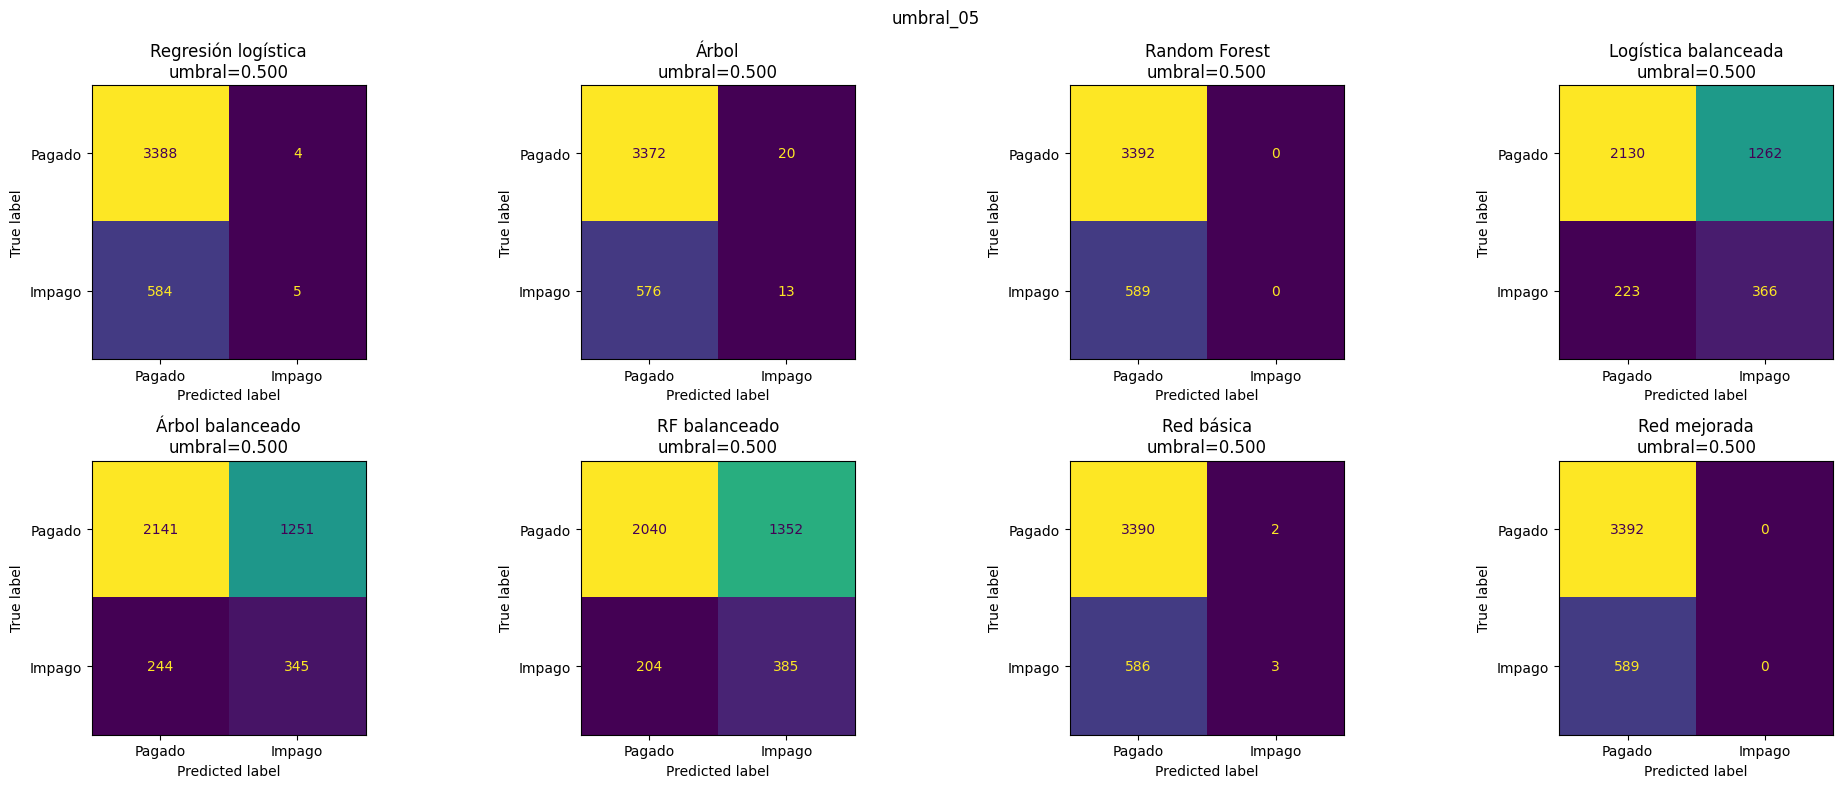
\includegraphics[width=\linewidth]{c38_0.png}
\end{figure}

Con el umbral de validación (Figura~\ref{fig:cmval}), la red mejorada detecta 296 de los 589 impagos con 870 falsas alarmas, y la logística balanceada detecta 278 con 774 falsas alarmas. La red básica detecta más impagos (338), pero con 1\,055 falsas alarmas. Ninguna matriz domina a las demás: elegir entre ellas depende del costo relativo de aprobar un préstamo que no se pagará frente a rechazar uno bueno.

\begin{figure}[H]
\caption{Matrices de confusión en prueba con el umbral elegido en validación}\label{fig:cmval}
\centering
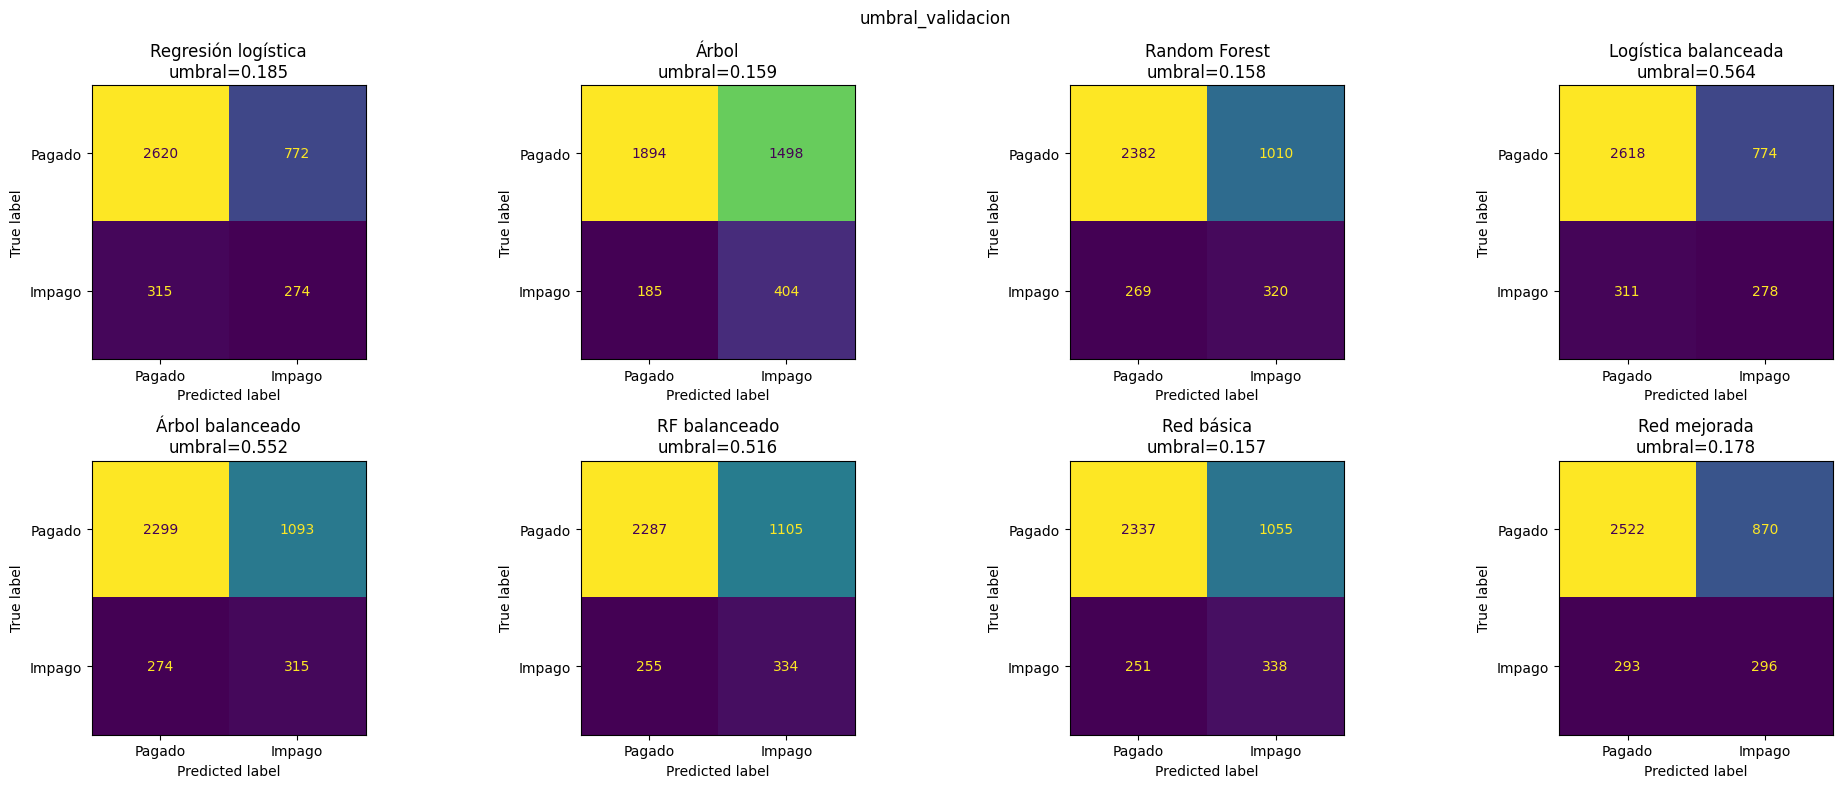
\includegraphics[width=\linewidth]{c38_1.png}
\end{figure}

Las curvas ROC y precisión--\textit{recall} (Figura~\ref{fig:rocpr}) están superpuestas para casi todos los modelos; solo los dos árboles quedan claramente por debajo. En la curva precisión--\textit{recall}, la red mejorada y la logística tienen algo más de precisión en la zona de \textit{recall} bajo, es decir, entre los préstamos que el modelo considera más riesgosos.

\begin{figure}[H]
\caption{Curvas ROC y precisión--\textit{recall} en prueba}\label{fig:rocpr}
\centering
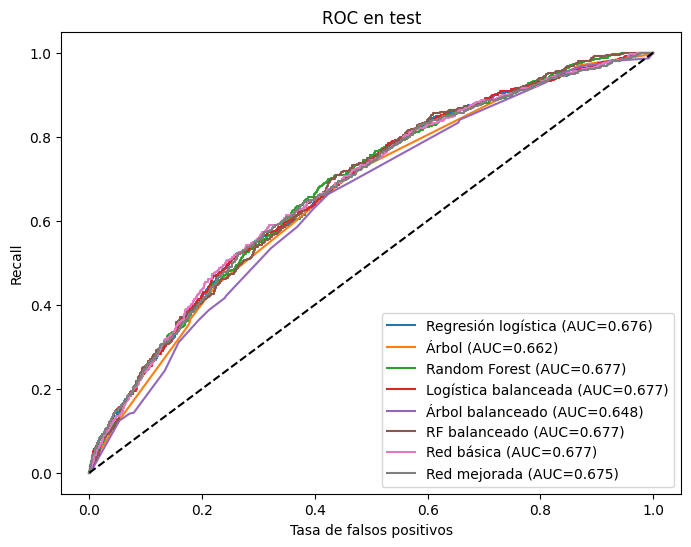
\includegraphics[width=0.49\linewidth]{c38_2.png}\hfill
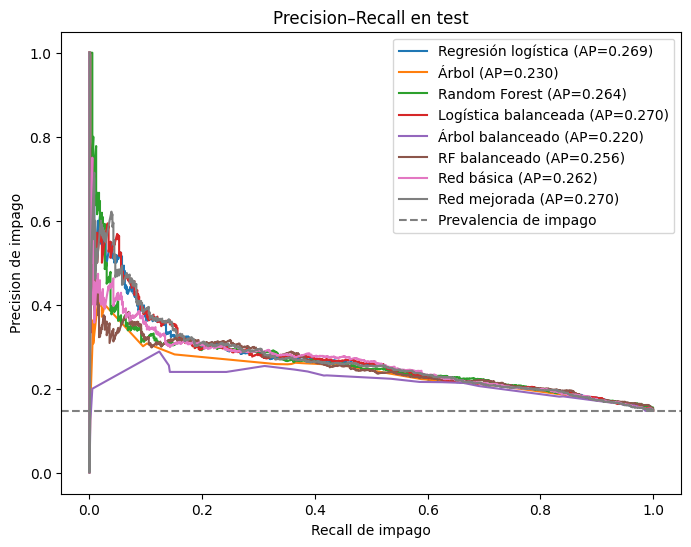
\includegraphics[width=0.49\linewidth]{c38_3.png}
\nota{La línea discontinua de la derecha es la prevalencia de impago (0.148), que es el AP de un clasificador aleatorio.}
\end{figure}

% =====================================================================
\section{Interpretabilidad}\label{sec:interp}

\subsection{Coeficientes de la regresión logística e importancias de árboles}

La regresión logística es interpretable de forma intrínseca: cada coeficiente es el cambio en el logaritmo de las probabilidades (\textit{log-odds}) de impago cuando la variable pasa del mínimo al máximo de entrenamiento (por el escalado a $[0,1]$), manteniendo las demás fijas. Las importancias del árbol y del \textit{Random Forest} miden cuánto reduce cada variable la impureza en las divisiones. La Tabla~\ref{tab:coef} muestra las 15 variables con mayor coeficiente absoluto.

\begin{table}[H]
\caption{Coeficientes de la regresión logística e importancias de árbol y Random Forest}\label{tab:coef}
\centering
\small
\begin{tabular}{lrrr}
\toprule
Variable & Coef. logística & Imp. árbol & Imp. RF \\
\midrule
\code{int\_rate}                         &  1.773 & 0.419 & 0.210 \\
\code{annual\_inc}                       & $-0.984$ & 0.149 & 0.084 \\
\code{delinq\_2yrs}                      & $-0.830$ & 0.000 & 0.004 \\
\code{application\_type\_Individual}     & $-0.595$ & 0.000 & 0.000 \\
\code{purpose\_small\_business}          &  0.568 & 0.066 & 0.032 \\
\code{loan\_amnt}                        & $-0.553$ & 0.045 & 0.033 \\
\code{term}                              &  0.526 & 0.050 & 0.169 \\
\code{grade\_A}                          & $-0.474$ & 0.129 & 0.101 \\
\code{purpose\_wedding}                  & $-0.418$ & 0.000 & 0.000 \\
\code{issue\_year}                       & $-0.352$ & 0.015 & 0.012 \\
\code{purpose\_car}                      & $-0.347$ & 0.000 & 0.000 \\
\code{home\_ownership\_MORTGAGE}         & $-0.345$ & 0.000 & 0.001 \\
\code{pub\_rec\_bankruptcies}            &  0.324 & 0.000 & 0.008 \\
\code{home\_ownership\_RENT}             & $-0.304$ & 0.000 & 0.001 \\
\code{purpose\_home\_improvement}        & $-0.292$ & 0.000 & 0.001 \\
\bottomrule
\end{tabular}
\nota{Coeficientes de la regresión logística sin pesos. Signo positivo: la variable aumenta el riesgo de impago.}
\end{table}

La tasa de interés es la variable dominante en los tres métodos. Le siguen el ingreso anual (a mayor ingreso, menor riesgo), el plazo de 60 meses y el grado A (que reduce el riesgo). Los préstamos para pequeños negocios elevan el riesgo, y los destinados a bodas, autos o mejoras del hogar lo reducen. Dos signos requieren cautela. El coeficiente negativo de \code{delinq\_2yrs} (morosidades pasadas) es contraintuitivo y probablemente refleja que su efecto ya está absorbido por la tasa y el grado, que el prestamista fija en función del historial. El de \code{application\_type\_Individual} afecta a casi todos los préstamos y funciona como un desplazamiento del intercepto. Los coeficientes describen asociaciones condicionadas a las demás variables, no efectos causales.

\subsection{SHAP sobre la red mejorada}

Para la red se usó SHAP con \code{KernelExplainer} (Lundberg \& Lee, 2017), que reparte la salida de un préstamo entre sus variables:
\begin{equation}\label{eq:shap}
f(x) = \mathbb{E}[f(X)] + \sum_{j=1}^{49}\phi_j(x),
\end{equation}
donde $f(x)$ es la salida de la red en \textit{log-odds}, $\mathbb{E}[f(X)]$ es la salida promedio sobre 50 préstamos de entrenamiento usados como referencia y $\phi_j$ es la contribución de la variable $j$. Se explicaron 200 préstamos de prueba (38 impagos). La referencia es $-1.851$ \textit{log-odds}, equivalente a una probabilidad de 0.136, y el error de aditividad de \eqref{eq:shap} fue 0.0000 en todos los casos.

\begin{figure}[H]
\caption{Valores SHAP de la red mejorada sobre 200 préstamos de prueba}\label{fig:beeswarm}
\centering
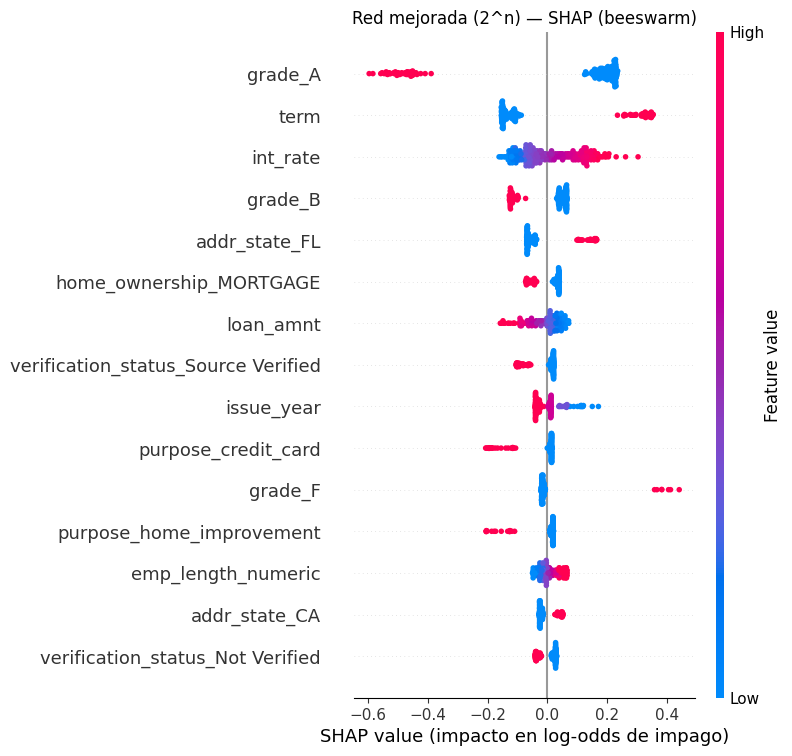
\includegraphics[width=0.7\linewidth]{c67_0.png}
\nota{Cada punto es un préstamo. El color indica el valor de la variable (rojo alto, azul bajo) y la posición horizontal su efecto en \textit{log-odds}: a la derecha aumenta el riesgo de impago.}
\end{figure}

La Figura~\ref{fig:beeswarm} muestra que la red se apoya sobre todo en el grado A (importancia media 0.269), el plazo (0.184), la tasa de interés (0.088) y el grado B (0.072). Las direcciones coinciden con la logística: tener grado A o B reduce el riesgo, y un plazo de 60 meses o una tasa alta lo aumentan. También aparecen el estado de Florida (aumenta el riesgo), tener hipoteca y préstamos más grandes (lo reducen) y el grado F (lo aumenta con fuerza en los pocos casos que lo tienen).

La red y la logística coinciden en las variables principales (tasa, plazo, grado y propósito \textit{small business}), pero las ordenan distinto: la red concentra el efecto en el grado crediticio y la logística en la tasa de interés. Ambas variables están muy correlacionadas, porque Lending Club asigna la tasa según el grado, y cada modelo reparte entre ellas el mismo efecto de forma diferente. El ingreso anual, segundo en la logística, no aparece entre las 15 primeras de SHAP.

\subsection{Explicación de un préstamo individual}

La Figura~\ref{fig:waterfall} explica el préstamo de prueba con mayor probabilidad de impago según la red: grado F, tasa de 18.3\,\%, plazo de 60 meses, propósito \textit{small business} y residencia en Florida. Partiendo de $-1.851$, las contribuciones suman $+1.197$ y llevan la salida a $-0.654$ \textit{log-odds}, es decir, una probabilidad de 0.342. Las mayores contribuciones son el propósito (+0.31), el grado F (+0.23), el plazo (+0.18) y no tener grado A (+0.15).

\begin{figure}[H]
\caption{Explicación SHAP del préstamo de prueba con mayor probabilidad de impago}\label{fig:waterfall}
\centering
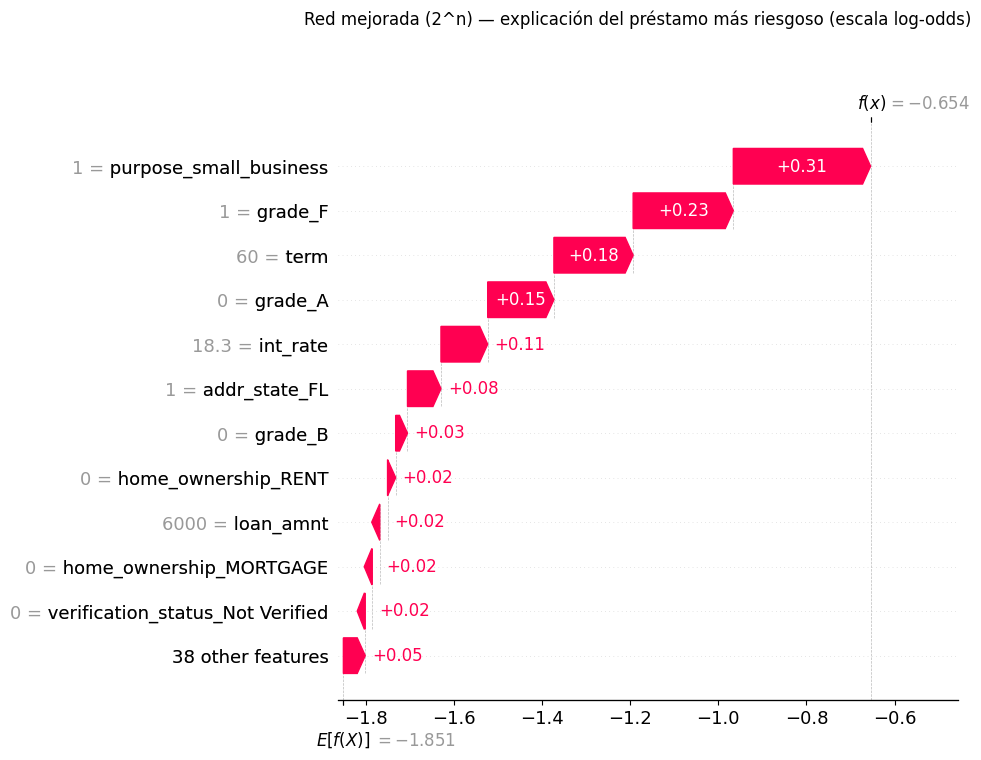
\includegraphics[width=0.75\linewidth]{c73_0.png}
\end{figure}

Dos observaciones. Primero, la probabilidad máxima que la red asigna en toda la prueba es 0.342, lo que explica por qué nunca supera el umbral de 0.5 y por qué su F1 con ese umbral es cero. Con el umbral de validación (0.178), este préstamo sí se marca como impago. Segundo, ese préstamo en realidad se pagó: un perfil de alto riesgo no garantiza el impago, y una probabilidad de 34\,\% significa que dos de cada tres préstamos parecidos se pagan.

% =====================================================================
\section{Discusión}\label{sec:discusion}

\paragraph{La red no supera a la regresión logística.} Con 49 variables tabulares, una relación con el riesgo cercana a la monotonía (más tasa, más plazo, peor grado implican más riesgo) y cerca de 13\,000 préstamos de entrenamiento, la frontera de decisión es casi lineal en el espacio de \textit{log-odds}. Una red de 20 capas puede representar esa frontera, pero no tiene estructura adicional que aprovechar. Que cinco modelos muy distintos converjan en un AUC de 0.675--0.677 indica que el límite está en la información disponible en las variables, no en el modelo.

\paragraph{La profundidad no ayudó.} El mejor AP de la búsqueda (0.2765) lo obtuvo la red de una sola capa con tanh, antes de las etapas de arquitectura. La consigna exigía comparar entre 5 y 100 capas, y al hacerlo el AP bajó. El procedimiento secuencial no permite volver atrás, de modo que la red final es más compleja y algo peor en validación que la mejor configuración vista.

\paragraph{Etapas sin la opción de conservar el valor previo.} En la etapa de \textit{dropout} no se incluyó el valor 0, y el procedimiento estaba obligado a elegir 0.25 o 0.50 aunque ambos empeoraran el AP (de 0.2721 a 0.2520). Algo similar ocurrió en la etapa de épocas: al desactivar el \textit{early stopping}, reemplazó una configuración con AP 0.2640 por otra con 0.2627. Incluir siempre la configuración vigente como candidata evitaría estos retrocesos.

\paragraph{El orden de las etapas sí importó.} Con el orden anterior, la red final se sobreajustaba (AUC 0.996 en entrenamiento y 0.582 en prueba). Con el nuevo orden, la tasa de aprendizaje baja (0.0001), el \textit{dropout} y la penalización L1 ya estaban fijados cuando se probaron las épocas, y la brecha entre entrenamiento y prueba quedó en 0.009. Además, fijar optimizador, tasa, lote y activación sobre la red de una capa abarató esas cuatro etapas. Queda el riesgo de que los valores elegidos con una capa no sean los mejores para 20 capas.

\paragraph{Limitaciones.} Toda la búsqueda usa una sola semilla, y diferencias de AP del orden de 0.001--0.005 están dentro de la variabilidad esperable entre corridas. El conjunto de validación se reutilizó para 43 decisiones y para elegir umbrales, lo que puede volverlo optimista; por eso la prueba se reservó hasta el final y sus métricas son algo menores (AUC 0.675--0.677 frente a 0.686--0.694). SGD se comparó con una tasa pensada para métodos adaptativos. Por último, SHAP se calculó con una muestra de 200 préstamos y una referencia de 50, y describe cómo usa la red las variables, no relaciones causales.

% =====================================================================
\section{¿Sirve la red neuronal para este problema?}\label{sec:sirve}

Que la red mejorada no supere a los modelos base no significa que la red no sirva para clasificar. Significa que, con estos datos, una red neuronal no tiene ventaja sobre modelos más simples. Esta sección separa ambas ideas y propone cómo continuar.

\subsection{La red sí aprende a clasificar}

Un clasificador aleatorio tendría un AUC de 0.5 y un AP igual a la prevalencia de impago (0.148). En prueba, la red mejorada alcanza un AUC de 0.675 y un AP de 0.270, casi el doble de precisión que el azar en la detección de impagos. Con el umbral elegido en validación identifica 296 de los 589 impagos de prueba (Figura~\ref{fig:cmval}), y su desempeño es estable entre entrenamiento, validación y prueba (Tabla~\ref{tab:tvt}). La red, por tanto, extrae una señal real de los datos.

\subsection{Por qué no supera a la regresión logística}

El indicio más importante es que cinco modelos de naturaleza muy distinta (regresión logística, árboles, \textit{Random Forest}, una red de una capa y una de 20 capas) convergen en el mismo AUC de prueba, entre 0.675 y 0.677. Cuando modelos tan diferentes llegan al mismo valor, el límite no lo impone el modelo, sino la información contenida en las variables. A ello se suman tres factores:

\begin{enumerate}
\item \textbf{Relación casi lineal y monótona.} Una tasa más alta, un plazo más largo o un peor grado crediticio implican más riesgo. La regresión logística captura esa relación de forma directa, y la red no encuentra estructura no lineal adicional que aprovechar.
\item \textbf{Tamaño de la muestra.} Con unos 13\,000 préstamos de entrenamiento y 49 variables, una red profunda no dispone de datos suficientes para sacar ventaja de su capacidad.
\item \textbf{Naturaleza tabular de los datos.} En datos tabulares, los modelos basados en árboles, especialmente los de \textit{gradient boosting}, suelen igualar o superar a las redes neuronales (Grinsztajn et al., 2022).
\end{enumerate}

\subsection{Valor del resultado para la tarea}

El objetivo de la tarea era diagnosticar y mejorar la red, y eso se cumplió: el F1 pasó de 0 a 0.34 y se eliminó el sobreajuste de la corrida anterior. Concluir que una red neuronal no supera a una regresión logística en este problema es un hallazgo legítimo. Además, en riesgo de crédito la interpretabilidad suele ser un requisito, y en ese aspecto la regresión logística tiene una ventaja clara a igual desempeño.

\subsection{Posibles cambios de estrategia}

Si el objetivo es mejorar el desempeño, se proponen los siguientes cambios, ordenados por el impacto esperado:

\begin{enumerate}
\item \textbf{Ingeniería de variables.} Si el límite está en la información disponible, la vía principal para superarlo es construir variables más informativas, por ejemplo cuota/ingreso, monto/ingreso o antigüedad del historial crediticio.
\item \textbf{\textit{Gradient boosting} como referencia.} Modelos como XGBoost o LightGBM son el estándar en riesgo de crédito con datos tabulares y constituyen una comparación más exigente.
\item \textbf{Ajustes a la búsqueda de la red.} Permitir redes de una o dos capas, que dieron el mejor AP (0.2765); incluir siempre la configuración vigente como candidata en cada etapa; y repetir las mejores configuraciones con varias semillas o validación cruzada, porque diferencias de AUC del orden de 0.002 probablemente se deben al azar del entrenamiento.
\item \textbf{Umbral según costos.} Elegir el umbral según el costo de aprobar un préstamo que no se pagará frente al de rechazar uno bueno, en lugar de maximizar el F1.
\end{enumerate}

Aun con estos cambios, se espera que la mejora en AUC sea moderada: con variables disponibles al momento de la solicitud, la capacidad de anticipar el impago parece tener un techo bajo, como sugiere la convergencia de todos los modelos.

% =====================================================================
\section{Conclusiones}\label{sec:conclusiones}

\begin{enumerate}
\item \textbf{Corregir el preprocesamiento era imprescindible.} El MinMaxScaler no llegaba a los modelos y la imputación usaba toda la base. Ahora todo se ajusta solo con entrenamiento y las redes aprenden una señal real (AUC $\approx$ 0.69 en validación).
\item \textbf{El desbalance explica el F1 = 0 del avance inicial.} Las redes respondían «pagado» para todos los préstamos. Los pesos de clase o un umbral elegido en validación lo resuelven y llevan el F1 a 0.34--0.36; combinarlos no suma, y los pesos no mejoran el AP.
\item \textbf{La búsqueda secuencial reordenada produjo una red estable.} La red final (20 capas de 64 neuronas tanh, Adam 0.0001, lote 32, \textit{dropout} 0.25, L1) ya no se sobreajusta: AUC de 0.683, 0.690 y 0.675 en entrenamiento, validación y prueba.
\item \textbf{La red no supera a los modelos base.} En prueba, la red mejorada (AUC 0.675, AP 0.270, F1 0.337), la red básica, la regresión logística y el \textit{Random Forest} están empatados. El modelo seleccionado solo con validación es la regresión logística balanceada (AUC 0.677, AP 0.270, F1 0.339), que además es más simple e interpretable.
\item \textbf{Las variables clave coinciden entre métodos.} Coeficientes logísticos, importancias de árboles y SHAP señalan la tasa de interés, el plazo, el grado crediticio y el propósito del préstamo como los principales determinantes del riesgo de impago.
\end{enumerate}

Como trabajo futuro se propone incluir siempre la configuración vigente como candidata en cada etapa, repetir las mejores configuraciones con varias semillas o validación cruzada, darle a SGD una tasa propia, y elegir el umbral según el costo real de cada tipo de error en lugar de maximizar el F1.

% =====================================================================
\section*{Referencias}
\addcontentsline{toc}{section}{Referencias}
\begingroup
\setlength{\parindent}{-1.25cm}
\setlength{\leftskip}{1.25cm}
\setlength{\parskip}{6pt}
\small

Glorot, X., \& Bengio, Y. (2010). Understanding the difficulty of training deep feedforward neural networks. En \textit{Proceedings of the Thirteenth International Conference on Artificial Intelligence and Statistics} (pp.~249--256). PMLR.

Goodfellow, I., Bengio, Y., \& Courville, A. (2016). \textit{Deep learning}. MIT Press.

Grinsztajn, L., Oyallon, E., \& Varoquaux, G. (2022). Why do tree-based models still outperform deep learning on typical tabular data? En \textit{Advances in Neural Information Processing Systems 35} (Datasets and Benchmarks Track).

Kingma, D. P., \& Ba, J. (2015). Adam: A method for stochastic optimization. En \textit{3rd International Conference on Learning Representations (ICLR)}.

Lundberg, S. M., \& Lee, S.-I. (2017). A unified approach to interpreting model predictions. En \textit{Advances in Neural Information Processing Systems 30} (pp.~4765--4774).

Pedregosa, F., Varoquaux, G., Gramfort, A., Michel, V., Thirion, B., Grisel, O., \ldots{} Duchesnay, É. (2011). Scikit-learn: Machine learning in Python. \textit{Journal of Machine Learning Research, 12}, 2825--2830.

Prechelt, L. (1998). Early stopping---but when? En G. B. Orr \& K.-R. Müller (Eds.), \textit{Neural networks: Tricks of the trade} (pp.~55--69). Springer.

Saito, T., \& Rehmsmeier, M. (2015). The precision-recall plot is more informative than the ROC plot when evaluating binary classifiers on imbalanced datasets. \textit{PLoS ONE, 10}(3), e0118432.

Srivastava, N., Hinton, G., Krizhevsky, A., Sutskever, I., \& Salakhutdinov, R. (2014). Dropout: A simple way to prevent neural networks from overfitting. \textit{Journal of Machine Learning Research, 15}, 1929--1958.

\endgroup

% =====================================================================
\newpage
\appendix
\section*{Anexo. Registro completo de la búsqueda}
\addcontentsline{toc}{section}{Anexo. Registro completo de la búsqueda}

\noindent La Tabla~\ref{tab:anexo} lista los 43 experimentos agrupados por etapa, en el orden de la búsqueda; dentro de cada etapa aparecen de mejor a peor AP. Todas las métricas son de validación.

{\footnotesize
\setlength{\tabcolsep}{3pt}
\begin{longtable}{llrrrrrrrr}
\caption{Experimentos de la búsqueda secuencial (validación)}\label{tab:anexo}\\
\toprule
Etapa & Valor & Exact. (\%) & F1 & F1 opt. & AP & AUC & Imp. pred. & Épocas & Seg. \\
\midrule
\endfirsthead
\toprule
Etapa & Valor & Exact. (\%) & F1 & F1 opt. & AP & AUC & Imp. pred. & Épocas & Seg. \\
\midrule
\endhead
\bottomrule
\endfoot
Balanceo & sin pesos & 85.05 & 0.004 & 0.360 & 0.2640 & 0.6860 & 7 & 10 & 8 \\
Balanceo & pesos balanceados & 66.75 & 0.355 & 0.359 & 0.2638 & 0.6835 & 1170 & 10 & 6 \\
Optimizador & adam & 85.18 & 0.004 & 0.361 & 0.2661 & 0.6888 & 3 & 10 & 6 \\
Optimizador & momentum & 85.21 & 0.000 & 0.361 & 0.2646 & 0.6880 & 0 & 60 & 38 \\
Optimizador & rmsprop & 85.21 & 0.004 & 0.360 & 0.2643 & 0.6873 & 2 & 10 & 8 \\
Optimizador & sgd & 85.21 & 0.000 & 0.349 & 0.2366 & 0.6660 & 0 & 100 & 63 \\
Tasa aprend. & 0.0001 & 85.18 & 0.004 & 0.366 & 0.2690 & 0.6895 & 3 & 48 & 29 \\
Tasa aprend. & 0.01 & 84.80 & 0.055 & 0.351 & 0.2683 & 0.6829 & 41 & 9 & 5 \\
Tasa aprend. & 0.001 & 85.18 & 0.004 & 0.361 & 0.2661 & 0.6888 & 3 & 10 & 7 \\
Batch & 32 & 85.18 & 0.004 & 0.365 & 0.2693 & 0.6899 & 3 & 32 & 33 \\
Batch & 64 & 85.18 & 0.004 & 0.366 & 0.2690 & 0.6895 & 3 & 48 & 29 \\
Batch & 128 & 85.18 & 0.004 & 0.362 & 0.2685 & 0.6892 & 3 & 58 & 22 \\
Activación & tanh & 85.31 & 0.021 & 0.366 & 0.2765 & 0.6940 & 7 & 63 & 61 \\
Activación & elu & 85.24 & 0.013 & 0.367 & 0.2757 & 0.6937 & 5 & 73 & 77 \\
Activación & sigmoid & 85.24 & 0.008 & 0.357 & 0.2738 & 0.6909 & 3 & 69 & 69 \\
Activación & relu & 85.18 & 0.004 & 0.365 & 0.2693 & 0.6899 & 3 & 32 & 36 \\
Capas & 20 & 85.12 & 0.078 & 0.346 & 0.2721 & 0.6836 & 43 & 38 & 109 \\
Capas & 5 & 85.24 & 0.017 & 0.351 & 0.2681 & 0.6852 & 7 & 14 & 20 \\
Capas & 10 & 85.15 & 0.008 & 0.355 & 0.2647 & 0.6814 & 6 & 21 & 40 \\
Capas & 50 & 85.21 & 0.000 & 0.353 & 0.2623 & 0.6817 & 0 & 19 & 119 \\
Capas & 100 & 85.21 & 0.000 & 0.276 & 0.1782 & 0.5716 & 0 & 7 & 96 \\
Neuronas & 64 & 85.12 & 0.078 & 0.346 & 0.2721 & 0.6836 & 43 & 38 & 109 \\
Neuronas & 128 & 85.21 & 0.000 & 0.348 & 0.2563 & 0.6810 & 0 & 8 & 35 \\
Neuronas & 512 & 85.21 & 0.000 & 0.354 & 0.2560 & 0.6836 & 0 & 10 & 377 \\
Neuronas & 32 & 85.24 & 0.004 & 0.329 & 0.2551 & 0.6672 & 1 & 8 & 24 \\
Neuronas & 256 & 85.21 & 0.000 & 0.350 & 0.2499 & 0.6754 & 0 & 6 & 64 \\
Distribución & Uniforme & 85.12 & 0.078 & 0.346 & 0.2721 & 0.6836 & 43 & 38 & 109 \\
Distribución & Embudo & 85.18 & 0.025 & 0.359 & 0.2636 & 0.6861 & 13 & 16 & 50 \\
Distribución & Cuello de botella & 85.12 & 0.008 & 0.357 & 0.2619 & 0.6860 & 7 & 13 & 41 \\
Distribución & Creciente & 85.18 & 0.004 & 0.327 & 0.2437 & 0.6582 & 3 & 7 & 25 \\
\textit{Dropout} & 0.25 & 85.21 & 0.000 & 0.351 & 0.2520 & 0.6737 & 0 & 25 & 94 \\
\textit{Dropout} & 0.5 & 85.21 & 0.000 & 0.271 & 0.1672 & 0.5431 & 0 & 6 & 27 \\
Regularización & L1 & 85.21 & 0.000 & 0.350 & 0.2640 & 0.6805 & 0 & 23 & 86 \\
Regularización & L2 & 85.21 & 0.000 & 0.348 & 0.2586 & 0.6820 & 0 & 27 & 101 \\
Regularización & sin & 85.21 & 0.000 & 0.351 & 0.2520 & 0.6737 & 0 & 25 & 91 \\
\textit{Early stopping} & patience=5 & 85.21 & 0.000 & 0.350 & 0.2640 & 0.6805 & 0 & 23 & 89 \\
\textit{Early stopping} & patience=10 & 85.21 & 0.000 & 0.350 & 0.2640 & 0.6805 & 0 & 28 & 111 \\
\textit{Early stopping} & patience=20 & 85.21 & 0.000 & 0.350 & 0.2640 & 0.6805 & 0 & 38 & 147 \\
\textit{Early stopping} & patience=50 & 85.21 & 0.000 & 0.350 & 0.2640 & 0.6805 & 0 & 68 & 251 \\
\textit{Early stopping} & sin parada & 85.21 & 0.000 & 0.357 & 0.2606 & 0.6905 & 0 & 100 & 371 \\
Épocas & 50 & 85.21 & 0.000 & 0.355 & 0.2627 & 0.6896 & 0 & 50 & 185 \\
Épocas & 100 & 85.21 & 0.000 & 0.357 & 0.2606 & 0.6905 & 0 & 100 & 376 \\
Épocas & 200 & 85.21 & 0.000 & 0.362 & 0.2594 & 0.6917 & 0 & 200 & 726 \\
\end{longtable}
}
\nota{F1 con umbral 0.5; «F1 opt.» con el umbral que maximiza F1 en validación. «Imp. pred.»: impagos predichos con umbral 0.5. El primer valor de cada etapa es el que se conservó.}

\end{document}
